\documentclass{standalone}

%----------------------------------------------------------------------------------------------%
%                                 Packages and basic declarations
%----------------------------------------------------------------------------------------------%

\usepackage{tikz}
\usepackage{verbatim}
\usepackage{pgf}
\usepackage{tikz}
\usepackage{mathrsfs}

\usetikzlibrary{arrows}



%----------------------------------------------------------------------------------------------%
%----------------------------------------------------------------------------------------------%
%                                            DOCUMENT STARTS
%----------------------------------------------------------------------------------------------%
%----------------------------------------------------------------------------------------------%

\begin{document}

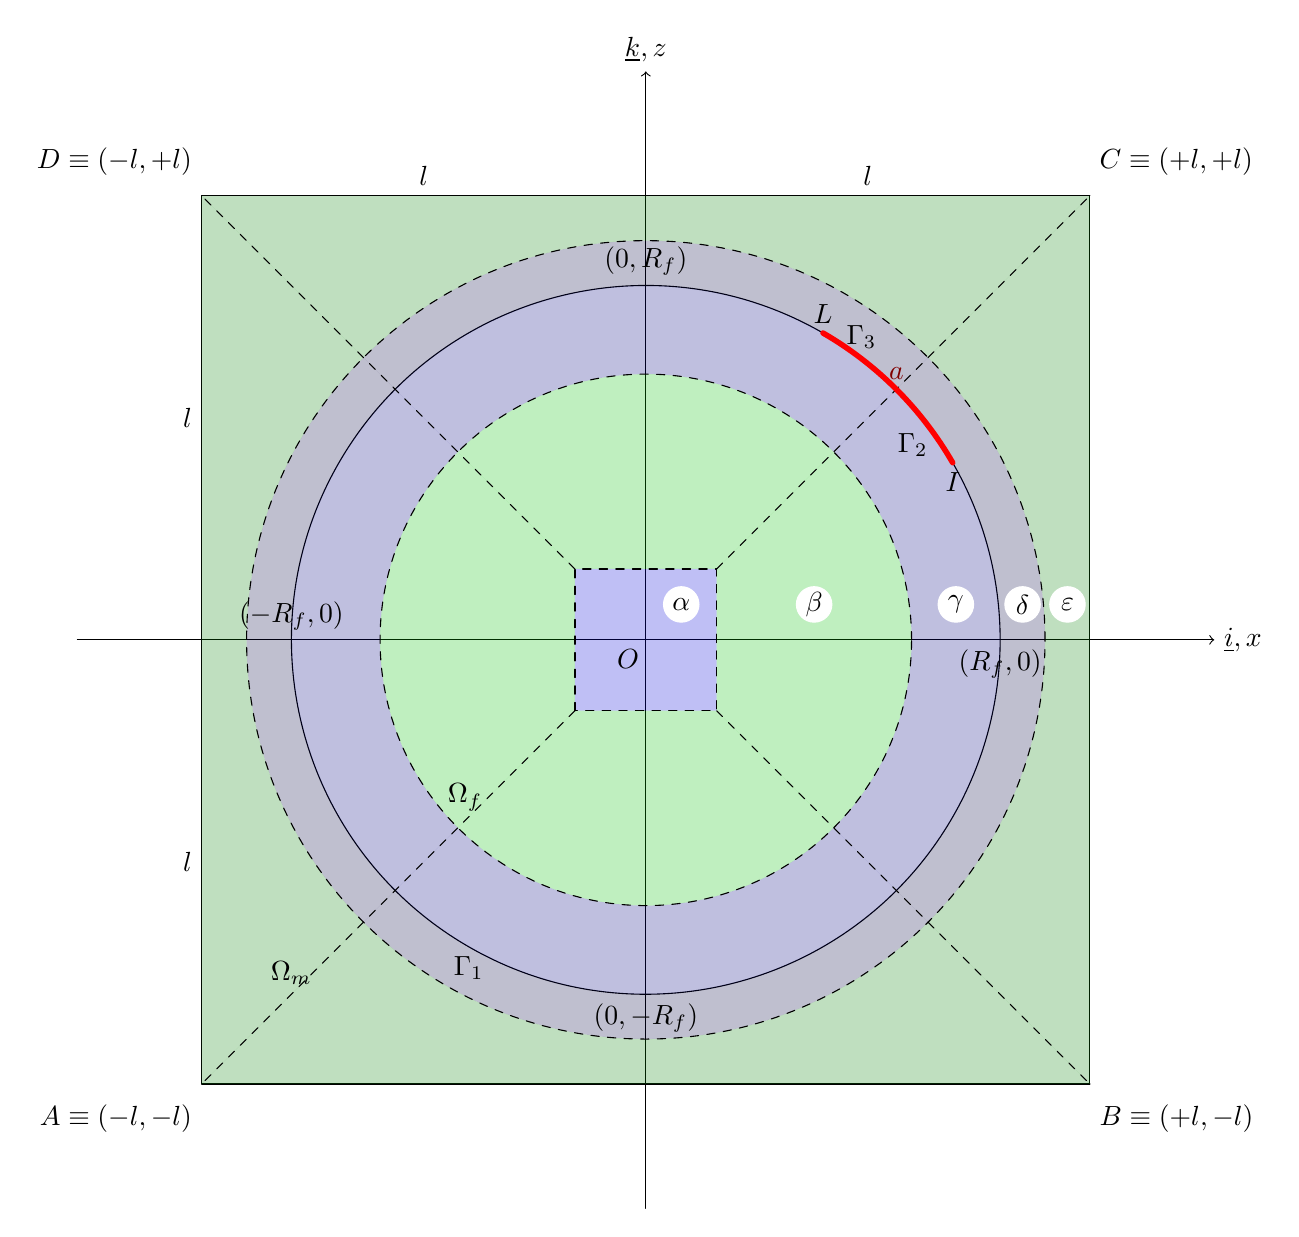
\begin{tikzpicture}[scale=4.5,cap=round,x=1cm,y=1cm]

%----------------------------------------------------------------------------------------------%
%                                          INPUT PARAMETERS
%----------------------------------------------------------------------------------------------%

\def\Rf{1}
\def\Vff{0.5}
\def\tratio{0.75}
\def\meshfacone{0.2}
\def\meshfactwo{0.75}
\def\meshfacthree{0.5}
\def\thetavalue{45}
\def\deltatheta{15}

%----------------------------------------------------------------------------------------------%
%                               Definition of dependent parameters
%----------------------------------------------------------------------------------------------%

\def\pivalue{3.141592653589793238462643383279502884197169399375105820974944592307816406286}

\newcommand{\half}[1]{
       0.5*#1
       }

\pgfmathsetmacro\l{0.5*\Rf*sqrt(\pivalue/\Vff)}

\def\domlim{1.28*\l}
\def\loadlim{1.197*\l}
\def\loadlabel{0.2*\Rf}
\def\cornerlabel{1.077*\l}

\def\thetabot{\thetavalue-\deltatheta}
\def\thetaup{\thetavalue+\deltatheta}

\def\thetahalfbot{\thetavalue-0.5*\deltatheta}
\def\thetahalfup{\thetavalue+0.5*\deltatheta}

\def\thetaround{360+\thetavalue-\deltatheta}
\def\thetadraw{0.25*\thetavalue}

\def\xM{0.9*\costheta*\Rf}
\def\yM{0.9*\sintheta*\Rf}

\pgfmathsetmacro\cosfourtyfive{cos(45)}
\pgfmathsetmacro\sinfourtyfive{sin(45)}

\pgfmathsetmacro\costheta{cos(\thetavalue)}
\pgfmathsetmacro\sintheta{sin(\thetavalue)}

\pgfmathsetmacro\costhetabot{cos(\thetabot)}
\pgfmathsetmacro\sinthetabot{sin(\thetabot)}

\pgfmathsetmacro\costhetaup{cos(\thetaup)}
\pgfmathsetmacro\sinthetaup{sin(\thetaup)}

\pgfmathsetmacro\costhetahalfbot{cos(\thetahalfbot)}
\pgfmathsetmacro\sinthetahalfbot{sin(\thetahalfbot)}

\pgfmathsetmacro\costhetahalfup{cos(\thetahalfup)}
\pgfmathsetmacro\sinthetahalfup{sin(\thetahalfup)}
  
\pgfmathsetmacro\yloadarrowone{\l+(\loadlim-\l)*0.2}
\pgfmathsetmacro\yloadarrowtwo{\l+2*(\loadlim-\l)*0.2}
\pgfmathsetmacro\yloadarrowthree{\l+3*(\loadlim-\l)*0.2}
\pgfmathsetmacro\yloadarrowfour{\l+4*(\loadlim-\l)*0.2}

\pgfmathsetmacro\ILsquared{(\costhetabot-\costhetaup)*(\costhetabot-\costhetaup)+(\sinthetabot-\sinthetaup)*(\sinthetabot-\sinthetaup))}
\pgfmathsetmacro\IMsquared{(\costhetabot-0.9*\costheta)*(\costhetabot-0.9*\costheta)+(\sinthetabot-0.9*\sintheta)*(\sinthetabot-0.9*\sintheta)}
\pgfmathsetmacro\IL{sqrt(\ILsquared)}
\pgfmathsetmacro\IM{sqrt(\IMsquared)}
\pgfmathsetmacro\angleM{asin(0.5*\IL/\IM)}

\def\crackstartangle{\thetavalue-\angleM}
\def\crackstopangle{\thetavalue+\angleM}

\pgfmathsetmacro\meshradiusone{\meshfactwo*\Rf}
\pgfmathsetmacro\meshradiustwo{\Rf+\meshfacthree*(\l-\Rf)}

\tikzstyle{axes}=[]

\draw (\costhetaup,\sinthetaup)arc (\thetaup:\thetaround:\Rf);

\begin{scope}[style=axes]
  \draw[->] (-\domlim,0) -- (\domlim,0) node[right] {$\underline{i}, x$};
  \draw[->] (0,-\domlim) -- (0,\domlim) node[above] {$\underline{k}, z$};
\end{scope}

\draw (-\l,-\l) -- (-\l,\l);
\draw (-\l,\l) -- (\l,\l) ;
\draw (\l,\l) -- (\l,-\l);
\draw (\l,-\l) -- (-\l,-\l);

\fill[fill=blue!85!black, fill opacity = 0.25] (-\meshfacone*\Rf,-\meshfacone*\Rf) -- (-\meshfacone*\Rf,\meshfacone*\Rf) -- (\meshfacone*\Rf,\meshfacone*\Rf) -- (\meshfacone*\Rf,-\meshfacone*\Rf) -- (-\meshfacone*\Rf,-\meshfacone*\Rf);
\filldraw[draw=white,fill=white] (0.5*\meshfacone*\Rf,0.5*\meshfacone*\Rf) circle(0.25*\meshfacone*\Rf);
\draw (0.5*\meshfacone*\Rf,0.5*\meshfacone*\Rf) node[black] {$\alpha$};

\fill[fill=green!75!black, fill opacity = 0.25] (-\meshfacone*\Rf,\meshfacone*\Rf) -- (\meshfacone*\Rf,\meshfacone*\Rf) -- (\meshradiusone*\cosfourtyfive,\meshradiusone*\cosfourtyfive) -- (\meshradiusone*\cosfourtyfive,\meshradiusone*\cosfourtyfive) arc(45:135:\meshradiusone) --  (-\meshfacone*\Rf,\meshfacone*\Rf);
\fill[fill=green!75!black, fill opacity = 0.25] (-\meshfacone*\Rf,\meshfacone*\Rf) -- (-\meshfacone*\Rf,-\meshfacone*\Rf) -- (-\meshradiusone*\cosfourtyfive,-\meshradiusone*\cosfourtyfive) -- (-\meshradiusone*\cosfourtyfive,-\meshradiusone*\cosfourtyfive) arc(225:135:\meshradiusone);
\fill[fill=green!75!black, fill opacity = 0.25] (-\meshfacone*\Rf,-\meshfacone*\Rf) -- (\meshfacone*\Rf,-\meshfacone*\Rf) -- (\meshradiusone*\cosfourtyfive,-\meshradiusone*\cosfourtyfive) -- (\meshradiusone*\cosfourtyfive,-\meshradiusone*\cosfourtyfive) arc(315:225:\meshradiusone);
\fill[fill=green!75!black, fill opacity = 0.25] (\meshfacone*\Rf,-\meshfacone*\Rf) -- (\meshfacone*\Rf,\meshfacone*\Rf) -- (\meshradiusone*\cosfourtyfive,\meshradiusone*\cosfourtyfive) -- (\meshradiusone*\cosfourtyfive,\meshradiusone*\cosfourtyfive) arc(45:-45:\meshradiusone);
\filldraw[draw=white,fill=white] (0.5*\meshfacone*\Rf+0.5*\meshradiusone,0.5*\meshfacone*\Rf) circle(0.25*\meshfacone*\Rf);
\draw (0.5*\meshfacone*\Rf+0.5*\meshradiusone,0.5*\meshfacone*\Rf) node[black] {$\beta$};

\fill[,fill=blue!50!black, fill opacity = 0.25] (-\meshradiusone*\cosfourtyfive,\meshradiusone*\cosfourtyfive) arc(135:45:\meshradiusone) -- (\Rf*\cosfourtyfive,\Rf*\cosfourtyfive) -- (\Rf*\cosfourtyfive,\Rf*\cosfourtyfive) arc(45:135:\Rf) --  (-\meshradiusone*\cosfourtyfive,\meshradiusone*\cosfourtyfive);
\fill[,fill=blue!50!black, fill opacity = 0.25] (\meshradiusone*\cosfourtyfive,\meshradiusone*\cosfourtyfive) arc(45:-45:\meshradiusone) -- (\Rf*\cosfourtyfive,-\Rf*\cosfourtyfive) -- (\Rf*\cosfourtyfive,-\Rf*\cosfourtyfive) arc(-45:45:\Rf) --  (\meshradiusone*\cosfourtyfive,\meshradiusone*\cosfourtyfive);
\fill[,fill=blue!50!black, fill opacity = 0.25] (\meshradiusone*\cosfourtyfive,-\meshradiusone*\cosfourtyfive) arc(315:225:\meshradiusone) -- (-\Rf*\cosfourtyfive,-\Rf*\cosfourtyfive) -- (-\Rf*\cosfourtyfive,-\Rf*\cosfourtyfive) arc(225:315:\Rf) --  (\meshradiusone*\cosfourtyfive,-\meshradiusone*\cosfourtyfive);
\fill[,fill=blue!50!black, fill opacity = 0.25] (-\meshradiusone*\cosfourtyfive,-\meshradiusone*\cosfourtyfive) arc(225:135:\meshradiusone) -- (-\Rf*\cosfourtyfive,\Rf*\cosfourtyfive) -- (-\Rf*\cosfourtyfive,\Rf*\cosfourtyfive) arc(135:225:\Rf) --  (-\meshradiusone*\cosfourtyfive,-\meshradiusone*\cosfourtyfive);
\filldraw[draw=white,fill=white] (0.5*\Rf+0.5*\meshradiusone,0.5*\meshfacone*\Rf) circle(0.25*\meshfacone*\Rf);
\draw (0.5*\Rf+0.5*\meshradiusone,0.5*\meshfacone*\Rf) node[black] {$\gamma$};

\fill[,fill=blue!25!black, fill opacity = 0.25] (-\Rf*\cosfourtyfive,\Rf*\cosfourtyfive) arc(135:45:\Rf) -- (\meshradiustwo*\cosfourtyfive,\meshradiustwo*\cosfourtyfive) -- (\meshradiustwo*\cosfourtyfive,\meshradiustwo*\cosfourtyfive) arc(45:135:\meshradiustwo) --  (-\Rf*\cosfourtyfive,\Rf*\cosfourtyfive);
\fill[,fill=blue!25!black, fill opacity = 0.25] (\Rf*\cosfourtyfive,\Rf*\cosfourtyfive) arc(45:-45:\Rf) -- (\meshradiustwo*\cosfourtyfive,-\meshradiustwo*\cosfourtyfive) -- (\meshradiustwo*\cosfourtyfive,-\meshradiustwo*\cosfourtyfive) arc(-45:45:\meshradiustwo) --  (\Rf*\cosfourtyfive,\Rf*\cosfourtyfive);
\fill[,fill=blue!25!black, fill opacity = 0.25] (\Rf*\cosfourtyfive,-\Rf*\cosfourtyfive) arc(315:225:\Rf) -- (-\meshradiustwo*\cosfourtyfive,-\meshradiustwo*\cosfourtyfive) -- (-\meshradiustwo*\cosfourtyfive,-\meshradiustwo*\cosfourtyfive) arc(225:315:\meshradiustwo) --  (\Rf*\cosfourtyfive,-\Rf*\cosfourtyfive);
\fill[,fill=blue!25!black, fill opacity = 0.25] (-\Rf*\cosfourtyfive,-\Rf*\cosfourtyfive) arc(225:135:\Rf) -- (-\meshradiustwo*\cosfourtyfive,\meshradiustwo*\cosfourtyfive) -- (-\meshradiustwo*\cosfourtyfive,\meshradiustwo*\cosfourtyfive) arc(135:225:\meshradiustwo) --  (-\Rf*\cosfourtyfive,-\Rf*\cosfourtyfive);
\filldraw[draw=white,fill=white] (0.5*\meshradiustwo+0.5*\Rf,0.5*\meshfacone*\Rf) circle(0.25*\meshfacone*\Rf);
\draw (0.5*\meshradiustwo+0.5*\Rf,0.5*\meshfacone*\Rf) node[black] {$\delta$};

\fill[fill=green!50!black, fill opacity = 0.25] (-\l,\l) -- (\l,\l) -- (\meshradiustwo*\cosfourtyfive,\meshradiustwo*\cosfourtyfive) -- (\meshradiustwo*\cosfourtyfive,\meshradiustwo*\cosfourtyfive) arc(45:135:\meshradiustwo) --  (-\l,\l);
\fill[fill=green!50!black, fill opacity = 0.25](-\l,-\l) -- (-\l,\l) -- (-\meshradiustwo*\cosfourtyfive,\meshradiustwo*\cosfourtyfive) -- (-\meshradiustwo*\cosfourtyfive,\meshradiustwo*\cosfourtyfive) arc(135:225:\meshradiustwo) --  (-\l,-\l);
\fill[fill=green!50!black, fill opacity = 0.25] (\l,-\l) -- (-\l,-\l) -- (-\meshradiustwo*\cosfourtyfive,-\meshradiustwo*\cosfourtyfive) -- (-\meshradiustwo*\cosfourtyfive,-\meshradiustwo*\cosfourtyfive) arc(225:315:\meshradiustwo) --  (\l,-\l);
\fill[fill=green!50!black, fill opacity = 0.25] (\l,\l) -- (\l,-\l) -- (\meshradiustwo*\cosfourtyfive,-\meshradiustwo*\cosfourtyfive) -- (\meshradiustwo*\cosfourtyfive,-\meshradiustwo*\cosfourtyfive) arc(-45:45:\meshradiustwo) --  (\l,\l);
\filldraw[draw=white,fill=white] (0.5*\l+0.5*\meshradiustwo,0.5*\meshfacone*\Rf) circle(0.25*\meshfacone*\Rf);
\draw (0.5*\l+0.5*\meshradiustwo,0.5*\meshfacone*\Rf) node[black] {$\varepsilon$};

\draw[dashed] (\meshfacone*\Rf,\meshfacone*\Rf) -- (\l,\l);
\draw[dashed] (-\meshfacone*\Rf,\meshfacone*\Rf) -- (-\l,\l);
\draw[dashed] (\meshfacone*\Rf,-\meshfacone*\Rf) -- (\l,-\l);
\draw[dashed] (-\meshfacone*\Rf,-\meshfacone*\Rf) -- (-\l,-\l);

\draw[dashed] (0,0) circle(\meshradiusone);
\draw[dashed] (0,0) circle(\meshradiustwo);

\draw[dashed] (-\meshfacone*\Rf,-\meshfacone*\Rf) rectangle (\meshfacone*\Rf,\meshfacone*\Rf);




\draw (-\l,\half{\l}) node[black,left] {$l$};
\draw (-\l,-\half{\l}) node[black,left] {$l$};
\draw (\half{\l},\l) node[black,above] {$l$};
\draw (-\half{\l},\l) node[black,above] {$l$};

\draw (\l,\cornerlabel) node[black,right] {$C\equiv\left(+l,+l\right)$};
\draw (-\l,\cornerlabel) node[black,left] {$D\equiv\left(-l,+l\right)$};

\draw (\l,-\cornerlabel) node[black,right] {$B\equiv\left(+l,-l\right)$};
\draw (-\l,-\cornerlabel) node[black,left] {$A\equiv\left(-l,-l\right)$};

\draw (0,\Rf) node[black,above] {$\left(0,R_{f}\right)$};
\draw (-\Rf,0) node[black,above] {$\left(-R_{f},0\right)$};
\draw (0,-\Rf) node[black,below] {$\left(0,-R_{f}\right)$};
\draw (\Rf,0) node[black,below] {$\left(R_{f},0\right)$};

\draw (-0.5\Rf,-0.5\Rf) node[black,above] {$\Omega_{f}$};
\draw (-\Rf,-\Rf) node[black,above] {$\Omega_{m}$};
\draw (-0.05,0) node[black,left,below] {$O$};
\draw (-\costhetaup*\Rf,-\sinthetaup*\Rf) node[black,below] {$\Gamma_{1}$};
\draw (\costhetabot*\Rf,\sinthetabot*\Rf) node[black,below] {$I$};
\draw (\costhetaup*\Rf,\sinthetaup*\Rf) node[black,above] {$L$};
\draw (\costheta*\Rf,\sintheta*\Rf) node[red!50!black,above] {$a$};
\draw (\costhetahalfup*\Rf,\sinthetahalfup*\Rf) node[black,above] {$\Gamma_{3}$};
\draw (0.95*\costhetabot*\Rf,1.1*\sinthetabot*\Rf) node[black,left] {$\Gamma_{2}$};

\draw[draw=red,line width=2pt](\costhetaup,\sinthetaup) arc(\thetaup:\thetabot:\Rf);



\end{tikzpicture}

\end{document}